\section{Proofs}
\label{app:proofs}

We write $\mu=\mathbb E[Y]$, $e=Y-m(Z)$, $\sigma^2(Z)=\mathbb E[e^2\mid Z]$, and $a=n/(n+N)$, with $n,N\to\infty$ and $N/n$ bounded away from zero, so that $a\in(0,1]$ is fixed.

\paragraph{Proposition 1 (unbiasedness).}
Let the labeled sample be split into $K$ folds at random, and let the learner be applied to the $K-1$ other folds. Out-of-fold values $\hat m_L(Z_i)$ and fold-averaged values $\hat m_U(\tilde Z_j)$ are evaluated at points independent of the fit, so each has expectation $\mu_{\hat m}=\mathbb E\,\hat m_{-k}(Z)$ (the fold models are exchangeable under random folds). Then
\[
\mathbb E\hat\theta=\mu+(1-a)\big(\mu_{\hat m}-\mu_{\hat m}\big)=\mu,
\]
for any learner with finite second moments. The estimator is unbiased in finite samples, not only asymptotically.

\paragraph{Proposition 2 (variance).}
Write $\delta=\tilde m-m$. Only the variance of $\delta$ enters, so its mean plays no role. The linearization gives $\hat\theta-\mu=(\bar Y_L-\mu)-(1-a)(\bar{\tilde m}_L-\mathbb E\tilde m)+(1-a)(\bar{\tilde m}_U-\mathbb E\tilde m)+o_p(n^{-1/2})$. The labeled and unlabeled terms are independent, so
\[
nV=\mathrm{Var}\{Y-(1-a)\tilde m\}+\frac{n(1-a)^2}{N}\mathrm{Var}(\tilde m).
\]
Since $n(1-a)^2/N=a(1-a)$ and $Y-(1-a)\tilde m=e+am-(1-a)\delta$ with $\mathbb E[e\mid Z]=0$,
\begin{align*}
nV&=\mathbb E\sigma^2+\mathrm{Var}\{am-(1-a)\delta\}+a(1-a)\mathrm{Var}(m+\delta)\\
&=\mathbb E\sigma^2+a^2\mathrm{Var}(m)-2a(1-a)\mathrm{Cov}(m,\delta)+(1-a)^2\mathrm{Var}(\delta)\\
&\quad+a(1-a)\{\mathrm{Var}(m)+2\mathrm{Cov}(m,\delta)+\mathrm{Var}(\delta)\}\\
&=\mathbb E\sigma^2+a\,\mathrm{Var}(m)+(1-a)\mathrm{Var}(\delta),
\end{align*}
because the $\mathrm{Cov}(m,\delta)$ terms cancel and $a^2+a(1-a)=a$, $(1-a)^2+a(1-a)=1-a$. The $L_2$ convergence of the learners implies convergence of the variance terms; a Lindeberg-type CLT applies under the finite-moment conditions.

\paragraph{Theorem 3 (bound and PPI++ gap).}
The observation for a unit is $O=(R,RY,Z)$ with $R\sim\mathrm{Bernoulli}(a)$ independent of $(Z,Y)$. Under missingness at random, the influence function of $\theta$ in the nonparametric model for $(Z,Y)$ is $\psi=\frac{R}{a}(Y-m(Z))+m(Z)-\theta$, which is the augmented estimator with the true nuisance (Robins, Rotnitzky and Zhao, 1994; Tsiatis, 2006). Its per-unit variance is $\mathbb E[\sigma^2]/a+\mathrm{Var}(m)$, and over $n+N$ units with $a(n+N)=n$ this gives $V^\star=\{\mathbb E\sigma^2+a\mathrm{Var}(m)\}/n$. The PPI++ estimator is the case $\tilde m=L$ (with $\mathbb E L=\mu$), so $\delta=L-m$ and $\mathrm{Var}(\delta)=\mathbb E(m-L)^2=\Delta_L$, because $\mathbb E(m-L)=0$. Subtracting from Proposition 2 gives $(1-a)\Delta_L/n$.

\paragraph{Corollaries 4–6.}
Corollary 4 (width ratio) follows from Theorem 3 with $\mathbb E(Y-L)^2+a\mathrm{Var}(L)=\mathbb E\sigma^2+a\mathrm{Var}(m)+(1-a)\Delta_L$, using $\mathrm{Var}(m)=\mathrm{Var}(L)+\Delta_L$ and $\mathbb E(Y-L)^2=\mathbb E\sigma^2+\Delta_L$. Corollary 5 (covariates): by the law of total variance, $\mathbb E\sigma^2(Z)=\mathbb E\sigma^2(Z^+)+\mathbb E\{m(Z^+)-m(Z)\}^2$ and $\mathrm{Var}\{m(Z)\}=\mathrm{Var}\{m(Z^+)\}-\mathbb E\{m(Z^+)-m(Z)\}^2$, so the difference of bounds is $(1-a)\mathbb E\{m(Z^+)-m(Z)\}^2/n$. Corollary 6 (learned calibrators) is Proposition 2 with $\tilde m$ and the sign of $\mathrm{Var}(\delta)-\Delta_L$.

\section{Implementation details}
\label{app:impl}

\paragraph{Estimators.}
All estimators use the same $(Y_L,f_L,f_U)$ or $(Y_L,Z_L,Z_U)$. Classical: $\bar Y_L$ with variance $s_L^2/n$. PPI: $\bar f_U+\overline{(Y-f)}_L$, variance $s^2_{f,U}/N+s^2_{r,L}/n$. PPI++: $\lambda^\star=\widehat{\mathrm{Cov}}(Y,f)/\{\widehat{\mathrm{Var}}(f)(1+n/N)\}$ with the variance from the plug-in formula. Stratified PPI \citep{fisch2024strat} with $\lambda_k=1$: quantile strata of the pooled prediction ($K=5$), point estimate $\bar u_U$ where $u=f+\bar r_{b(f)}$ and $\bar r_b$ is the labeled stratum residual mean (falling back to the pooled residual mean when a stratum has fewer than two labels); variance $\widehat{\mathrm{Var}}_U(u)/N+\widehat{\mathrm{Var}}_L(Y-u)/n$. Cross-fitted calibration: $K=5$ folds, estimator and variance as in \cref{eq:common,eq:cfvar}. Spline learner: \texttt{SplineTransformer(degree=3, n\_knots=5)} with standardization and ridge penalty $\alpha=1$, applied to each column of $Z$ additively. Boosting: \texttt{HistGradientBoostingRegressor(max\_depth=3, learning\_rate=0.05, max\_iter=200, min\_samples\_leaf=10)}. Linear: ordinary least squares.

\paragraph{Learner choice.}
The development run used 100 replications per cell with seeds disjoint from the reported ones. For each learner we computed the mean width ratio to PPI++ over all cells of each scenario, and then averaged over scenarios. The spline gave $0.967$, boosting $0.978$, and linear $1.009$. The spline won in the binary, covariate, and heavy-tailed scenarios; boosting was marginally better in the nonlinear scenario ($0.813$ vs $0.826$). Coverage across learners and cells was between $0.89$ and $1.00$.

\paragraph{Sampling.}
Synthetic: labeled and unlabeled samples are drawn independently from the same population; the truth is computed once with $10^7$ draws. Real: indices are drawn independently with replacement from each pool (so the sampling model is i.i.d.\ by construction), and the target is the pool mean.

\section{Additional tables and figures}
\label{app:tables}

\begin{table*}[t]
  \centering
  \caption{Synthetic results, $N=4n$, \REPSSYN{} replications per cell. Columns give the width ratio vs PPI++ for the spline calibrator (CF spline), its coverage, boosting, stratified PPI, PPI, the efficient bound (oracle calibrator, from population constants), and the coverage of PPI++.}
  \label{tab:synth}
  \small
  \begin{tabular}{llccccccc}
\toprule
Scenario & $n$ & CF spline & CF cov. & CF boosting & Strat. PPI & PPI & Bound & PPI++ cov. \\
\midrule
linear calibrator & 50 & 1.162 & 0.938 & 1.192 & 1.098 & 1.299 & 1.000 & 0.944 \\
 & 200 & 1.051 & 0.944 & 1.048 & 1.108 & 1.309 & 1.000 & 0.946 \\
 & 1000 & 1.011 & 0.944 & 1.013 & 1.110 & 1.309 & 1.000 & 0.952 \\
nonlinear calibration & 50 & 0.829 & 0.950 & 0.855 & 0.986 & 1.118 & 0.756 & 0.950 \\
 & 200 & 0.807 & 0.968 & 0.795 & 0.999 & 1.110 & 0.756 & 0.960 \\
 & 1000 & 0.824 & 0.954 & 0.771 & 1.002 & 1.110 & 0.756 & 0.944 \\
binary outcome & 50 & 1.021 & 0.938 & 1.051 & 0.991 & 1.018 & 0.979 & 0.938 \\
 & 200 & 0.991 & 0.968 & 1.026 & 1.007 & 1.015 & 0.979 & 0.964 \\
 & 1000 & 0.982 & 0.936 & 0.997 & 1.010 & 1.013 & 0.979 & 0.936 \\
covariate beyond $f$ & 50 & 0.891 & 0.946 & 1.012 & 1.009 & 1.036 & 0.761 & 0.934 \\
 & 200 & 0.820 & 0.970 & 0.831 & 1.022 & 1.028 & 0.761 & 0.944 \\
 & 1000 & 0.817 & 0.950 & 0.782 & 1.025 & 1.026 & 0.761 & 0.962 \\
heavy-tailed noise & 50 & 0.899 & 0.946 & 0.929 & 0.987 & 1.084 & 0.860 & 0.924 \\
 & 200 & 0.883 & 0.946 & 0.892 & 0.999 & 1.077 & 0.860 & 0.944 \\
 & 1000 & 0.894 & 0.962 & 0.872 & 1.001 & 1.071 & 0.860 & 0.962 \\
\bottomrule
\end{tabular}

\end{table*}

\begin{table*}[t]
  \centering
  \caption{Calibrator sensitivity on the public pools at $n=200$, $N=4n$: width ratio vs PPI++ (with covariate adjustment in $f{+}X$ rows). Spline is the primary calibrator; boosting and linear are alternatives; stratified PPI and PPI are shown for comparison.}
  \label{tab:realsens}
  \small
  \begin{tabular}{llcccccc}
\toprule
Pool & Info & CF spline & CF boosting & CF linear & Strat. PPI & PPI & Classical \\
\midrule
galaxies & f & 1.015 & 1.053 & 1.007 & 1.019 & 1.031 & 1.340 \\
forest & f & 1.015 & 1.047 & 1.010 & 1.010 & 1.025 & 1.148 \\
gene expr. & f & 1.014 & 1.019 & 1.003 & 1.081 & 1.012 & 1.967 \\
alphafold & f & 1.015 & 1.047 & 1.006 & 1.026 & 1.026 & 1.475 \\
alphafold & f+X & 1.021 & 1.051 & 1.013 & 1.027 & 1.027 & 1.469 \\
census income & f & 1.034 & 1.068 & 1.018 & 1.012 & 1.008 & 1.214 \\
census income & f+X & 1.039 & 1.089 & 1.021 & 1.013 & 1.008 & 1.220 \\
census health & f & 1.014 & 1.056 & 1.006 & 1.016 & 1.025 & 1.292 \\
census health & f+X & 1.015 & 1.069 & 1.008 & 1.016 & 1.024 & 1.297 \\
census educ. & f & 1.021 & 1.055 & 1.010 & 1.012 & 1.020 & 1.218 \\
census educ. & f+X & 1.035 & 1.083 & 1.017 & 1.011 & 1.022 & 1.214 \\
\bottomrule
\end{tabular}

\end{table*}

\begin{table}[t]
  \centering
  \caption{Pool-level constants. $\kappa=\Delta_L/\mathbb E(Y-L)^2$ is the nonlinear share of the linear residual variance (an upper estimate, since $\Delta_L$ is estimated from a cross-fitted gradient-boosting calibrator and inherits its error). $R^2_{\rm lin}$ and $R^2_{\rm nl}$ are out-of-fold fits. The last three columns give the efficient-bound width ratio vs PPI++ at each $a$, computed from $\Delta_L$, $\mathbb E(Y-L)^2$ and $\mathrm{Var}(L)$.}
  \label{tab:pool}
  \small
  \begin{tabular}{llrrrrrrr}
\toprule
Pool & Info & $M$ & $R^2_{\rm lin}$ & $R^2_{\rm nl}$ & $\kappa$ & $a{=}\tfrac12$ & $a{=}\tfrac15$ & $a{=}\tfrac1{17}$ \\
\midrule
galaxies & f & 16743 & 0.549 & 0.543 & 0.008 & 0.999 & 0.997 & 0.996 \\
forest & f & 1596 & 0.289 & 0.248 & 0.054 & 0.989 & 0.980 & 0.975 \\
gene expr. & f & 61150 & 0.928 & 0.930 & 0.031 & 0.999 & 0.997 & 0.992 \\
alphafold & f & 10802 & 0.664 & 0.664 & 0.029 & 0.996 & 0.992 & 0.988 \\
alphafold & f+X & 10802 & 0.665 & 0.666 & 0.045 & 0.994 & 0.987 & 0.981 \\
census income & f & 380091 & 0.369 & 0.372 & 0.006 & 0.999 & 0.998 & 0.997 \\
census income & f+X & 380091 & 0.370 & 0.375 & 0.013 & 0.997 & 0.995 & 0.994 \\
census health & f & 318215 & 0.500 & 0.500 & 0.002 & 1.000 & 0.999 & 0.999 \\
census health & f+X & 318215 & 0.500 & 0.500 & 0.003 & 0.999 & 0.999 & 0.999 \\
census educ. & f & 318215 & 0.392 & 0.392 & 0.002 & 1.000 & 0.999 & 0.999 \\
census educ. & f+X & 318215 & 0.392 & 0.393 & 0.005 & 0.999 & 0.998 & 0.998 \\
\bottomrule
\end{tabular}

\end{table}

\begin{table*}[t]
  \centering
  \caption{Oracle-calibrator Monte Carlo check at $n=200$, $N=4n$ ($3000$ replications): Monte Carlo SD of the estimate and of its width ratio vs PPI++, next to the predictions of Proposition 2. $\mathrm{Var}(\delta)$ is the calibrator error variance added to the oracle.}
  \label{tab:theory}
  \small
  \begin{tabular}{lllrrrrrr}
\toprule
Scenario & Info & Calibrator error & $\Delta_L$ & MC sd & Pred.\ sd & MC ratio & Pred.\ ratio & Coverage \\
\midrule
linear calibrator & f & $\mathrm{Var}(\delta){=}0.00$ & 0.000 & 0.0746 & 0.0750 & 1.001 & 1.000 & 0.953 \\
linear calibrator & f & $\mathrm{Var}(\delta){=}0.04$ & 0.000 & 0.0757 & 0.0761 & 1.015 & 1.014 & 0.953 \\
nonlinear calibration & f & $\mathrm{Var}(\delta){=}0.00$ & 0.426 & 0.0472 & 0.0477 & 0.757 & 0.756 & 0.948 \\
nonlinear calibration & f & $\mathrm{Var}(\delta){=}0.04$ & 0.426 & 0.0489 & 0.0493 & 0.784 & 0.782 & 0.947 \\
binary outcome & f & $\mathrm{Var}(\delta){=}0.00$ & 0.007 & 0.0255 & 0.0259 & 0.980 & 0.979 & 0.954 \\
binary outcome & f & $\mathrm{Var}(\delta){=}0.04$ & 0.007 & 0.0286 & 0.0288 & 1.091 & 1.090 & 0.957 \\
covariate beyond $f$ & f & $\mathrm{Var}(\delta){=}0.00$ & 0.000 & 0.0692 & 0.0689 & 1.002 & 1.000 & 0.949 \\
covariate beyond $f$ & f & $\mathrm{Var}(\delta){=}0.04$ & 0.000 & 0.0700 & 0.0701 & 1.018 & 1.017 & 0.954 \\
 & X & $\mathrm{Var}(\delta){=}0.00$ & -- & 0.0517 & 0.0525 & 0.762 & 0.761 & 0.954 \\
 & X & $\mathrm{Var}(\delta){=}0.04$ & -- & 0.0536 & 0.0540 & 0.784 & 0.783 & 0.952 \\
heavy-tailed noise & f & $\mathrm{Var}(\delta){=}0.00$ & 0.426 & 0.0677 & 0.0695 & 0.852 & 0.860 & 0.955 \\
heavy-tailed noise & f & $\mathrm{Var}(\delta){=}0.04$ & 0.426 & 0.0687 & 0.0707 & 0.867 & 0.874 & 0.956 \\
\bottomrule
\end{tabular}

\end{table*}

\begin{figure}[t]
  \centering
  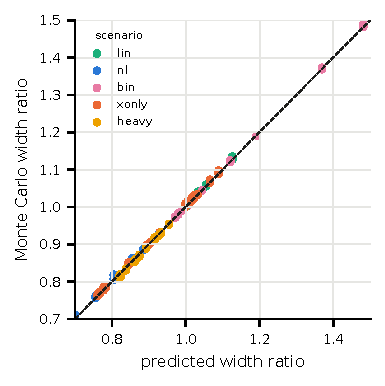
\includegraphics[width=\columnwidth]{figures/fig_theory.pdf}
  \caption{Predicted vs Monte Carlo width ratio for all oracle calibrators in \cref{tab:theory} and all $(n,N/n)$ cells. Dashed: identity.}
  \label{fig:theory}
\end{figure}

\section{Reproducibility checklist}
\label{app:checklist}

ICML 2026 does not require a separate checklist at submission (its call asks for supporting, reproducible evidence and a broader impact statement), but we give the relevant information here.

\begin{itemize}
  \item \textbf{Code and environment.} Python 3.11.2 with numpy 2.4.6, scipy 1.17.1, pandas 3.1.1, scikit-learn 1.9.1, ppi-python 0.2.3 (tag \texttt{v0.2.3}), gdown 6.5.1, matplotlib 3.11.2 (pinned in \texttt{requirements.txt}). Commands and runtime estimates are in \texttt{README.md}.
  \item \textbf{Data.} The nine \texttt{ppi-python} example pools, downloaded by the package loader; seven are used. No external data beyond these were used.
  \item \textbf{Seeds.} Every cell has a deterministic seed derived from its indices (see \texttt{README.md}).
  \item \textbf{Compute.} A 4-CPU quota. Total pipeline time \TOTALTIME{} (synthetic main about 100 min, real main about 165 min, pool and theory checks about 10 min).
  \item \textbf{Table and figure provenance.} \cref{tab:synth}: \texttt{run\_synth.py}, \texttt{summarize.py}, \texttt{make\_tables.py}. \cref{tab:real}, \cref{tab:realsens}, \cref{tab:pool}: \texttt{run\_real.py}, \texttt{theory\_pool.py}, \texttt{summarize.py}, \texttt{make\_tables.py}. \cref{tab:theory}, \cref{fig:theory}: \texttt{theory\_check.py}, \texttt{make\_tables.py}, \texttt{make\_figures.py}. \cref{fig:synth}: \texttt{make\_figures.py} (from \texttt{synth\_main\_summary.csv} and \texttt{theory\_check.csv}). \cref{fig:real}: \texttt{make\_figures.py} (from \texttt{real\_main.csv} and \texttt{theory\_pool.csv}). The large-$n$ extension: \texttt{run\_real.py --ns 5000 20000 --ratios 4} on four pools.
  \item \textbf{Failed or abandoned runs.} The first development run used a naive stratified-PPI variance and was discarded for that method (its rows are not used). The dev run for the learner choice used 100 replications per cell instead of 200 because of the CPU quota. No other runs were discarded.
\end{itemize}

\section{Literature check}
\label{app:lit}

References were checked against arXiv and publisher metadata pages. Starter references (PPI, PPI++, cross-PPI, active inference, StratPPI, DML) were read from their abstracts and, for StratPPI, from the full text to confirm the estimator form. For the three classical references (Zhang, Brown and Cai 2019; Chakrabortty and Cai 2018; Robins et al. 1994) we confirmed bibliographic metadata but not every claim in their full text, so we cite them only for the setting they treat. Incidental search results for unrelated semi-supervised papers were seen as snippets during this check; none was opened in full or used. We did not search for, open, or use any paper on shortening prediction-powered intervals under fixed labeled, unlabeled and predictor budgets beyond the starter list.
